\section{Graphs}
A \textit{graph} is an ordered pair $G = (V,E)$ comprising of a set of vertices $V$ and a set of edges $E$.  
An edge is a two element subset of $V$.
Note that with this definition of an edge it is not possible to have one element subset of $V$ as an edge (sometimes referred to as a self-adjacent edge or loop).
The \textit{degree} of a vertex $v$ is the number of edges that $v$ is an element of.
% and is denoted as ``V choose two'', ${V \choose 2}$.
% Each edge $e \in E$ is an unordered pair of vertices $\curlybraces{u,v} \in E$.  
Vertices are said to be \textit{adjacent} if they form an edge in $E$.  
\textit{Neighbors} of a vertex $v$ are the vertices adjecent to $v$.
%Vertices that are adjacent to themselves are \textit{self-adjacent}, i.e. $u = v$ for $\curlybraces{u,v} \in E$.  
Edges are said to be adjacent if they share a vertex.  

%When an edge is a member of $E$ multiple times,  then we say that the graph is a \textit{multigraph}.   
A \textit{simple graph} has no self-adjacent vertices.
In this thesis every graph is a simple graph.
Given a graph $G = (V,E)$, a set of vertices $S \subset V$ is \textit{independent} if no two vertices in $S$ are joined by an edge. 
A \textit{vertex cover} of a graph $G = (V,E)$  is a set of vertices $S \subset V$ if every edge $e \in E$, has at least one end corresponding in $S$.
If $G' = (V',E')$ is a graph such that $V' \subset V$ and $E' \subset E$, then $G'$ is a \textit{subgraph} of $G$.

To formally show when two graphs are the same, we use the concept of graph isomorphism.
%For graph equivalency, we need to define an isomorphism for graphs.  
Two graphs $G_1 =(V_1,E_1)$ and $G_2 = (V_2,E_2) $ are \textit{isomorphic} if there exists a bijective function $f: V_1 \mapsto V_2$ such that for any two vertices $u,v \in V_1$, we have $\{u, v\} \in E_1$ if and only if $(f(u),f(v)) \in E_2$. 
See an example in Table \ref{table:ch1-graph-1} and Figure \ref{fig:configuration-3}.
%Given two graphs $G_1 =(V_1,E_1)$ and $G_2 = (V_2,E_2) $, a \textit{graph isomorphism} is a bijective function $f: V_1 \mapsto V_2$ such that for any two vertices $u,v \in V_1$, we have $\{u, v\} \in E_1$, if and only if $(f(u),f(v)) \in E_2$. 
\begin{table}[!htbp]\label{table:ch1-graph-1}
\begin{center}
$$\begin{array}{|c|c|c|}\hline
\text{Graph}&\text{Vertices}&\text{Edges}\\\hline
G_1&\left\lbrace a,b,c,d,e \right\rbrace & \left\lbrace (a,b),(b,c),(c,d),(d,e),(e,a) \right\rbrace 
\\\hline
G_2&\left\lbrace 1,2,3,4,5 \right\rbrace & \left\lbrace (1,2),(2,3),(3,4),(4,5),(5,1) \right\rbrace 
\\\hline
\end{array} $$
\caption{Two graphs that are isomorphic with the alphabetical isomorphism $f(a)=1$, $f(b)=2$, $f(c) 
= 3$, $f(d)=4$, $f(e)=5$.}
\end{center} 
\end{table}

\begin{figure}[!htbp]
\begin{center}
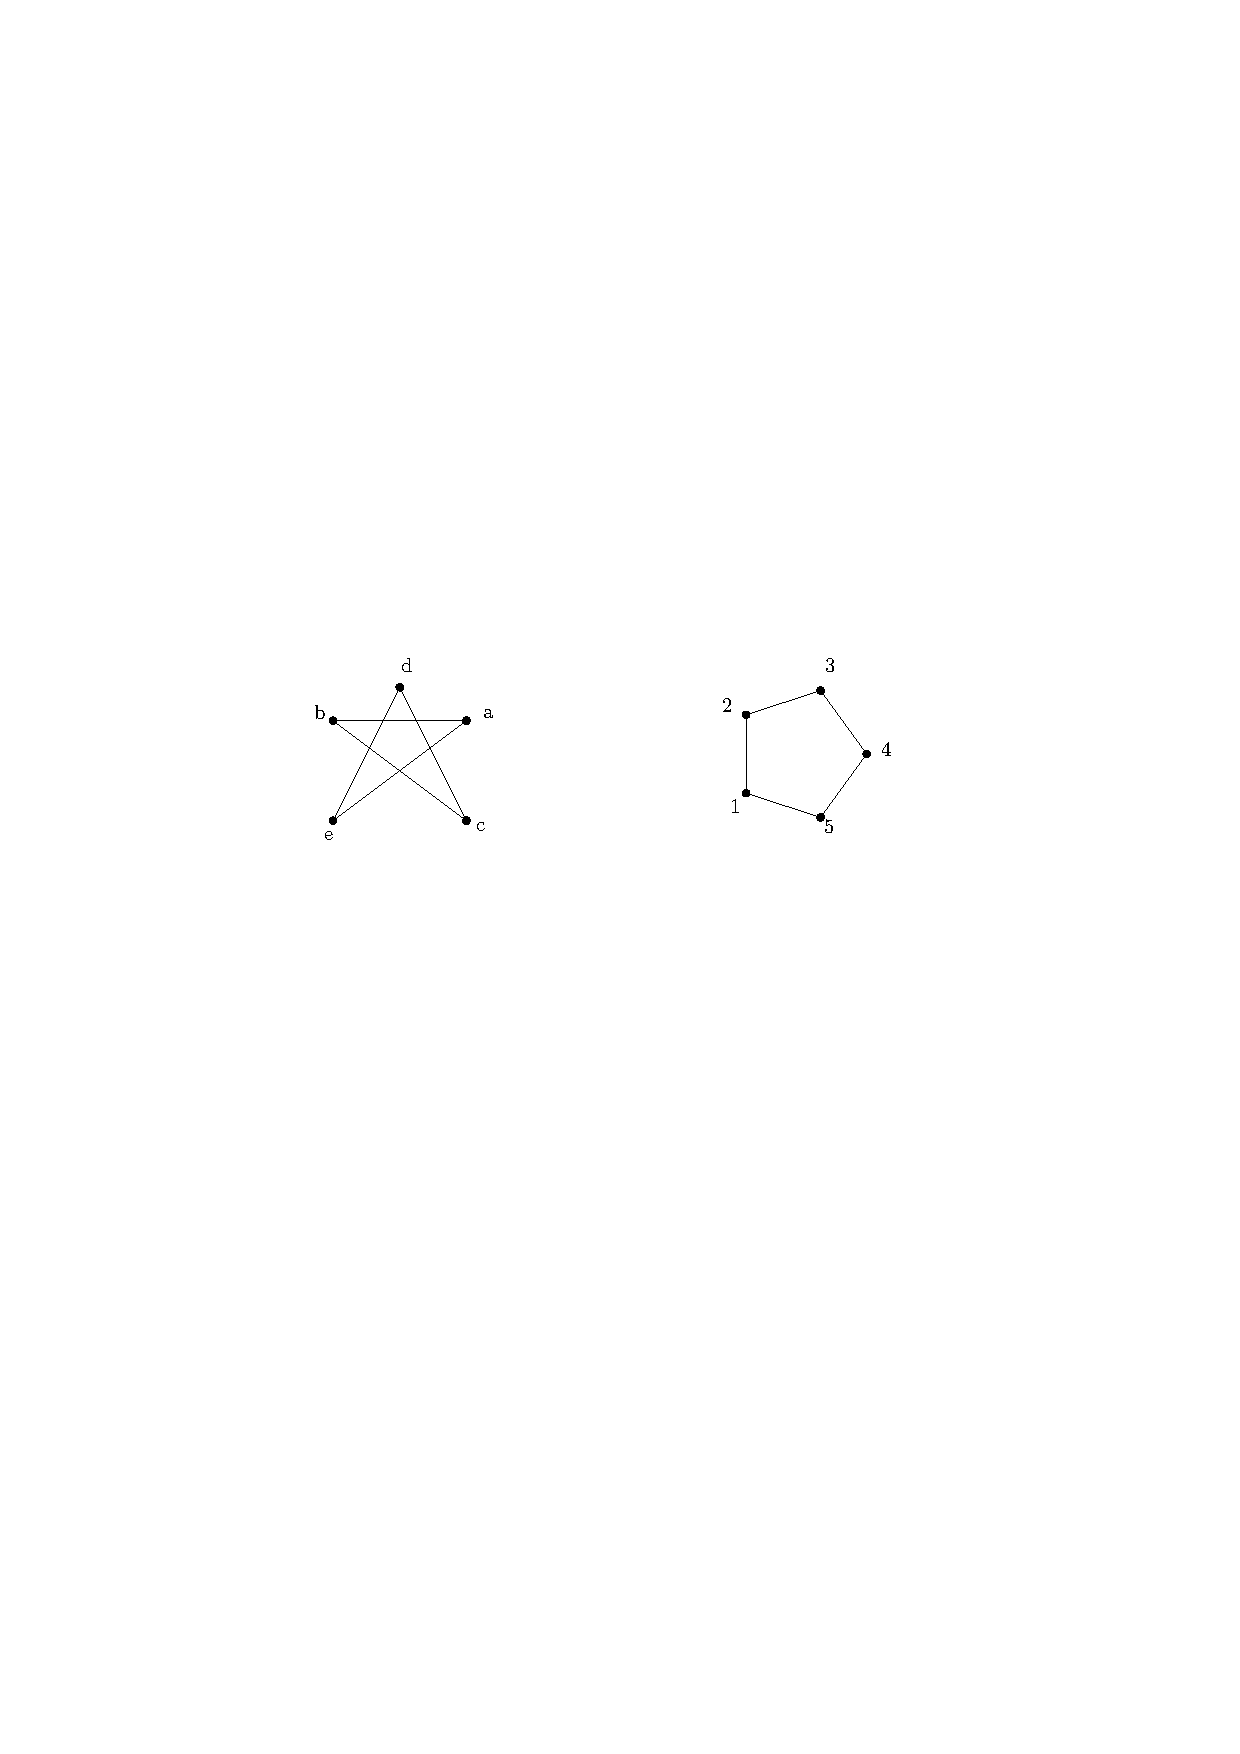
\includegraphics[scale=1]{graphics/graphIsomorphismExample.pdf}
\end{center} 
\caption{This figure depicts the graph isomorphism shown in Table \ref{table:ch1-graph-1} between $V_1$ and $V_2$.}
\label{fig:configuration-3}
\end{figure}

To visualize a graph, $G$, we create a drawing $\Gamma$, of $G$.  
The \textit{drawing} of a graph $G=(V,E)$ is an injective mapping $\Pi : V \mapsto \bbR^{2}$ which maps vertices to distinct points in the plane and for each edge $\curlybraces{u,v} \in E$, a continuous, injective mapping $c_{u,v}:[0,1]\mapsto \bbR^2$ such that $c_{u,v}(0) = \Pi(u)$, $c_{u,v}(1) = \Pi(v)$ , and the curve $c_{u,v}$ does not pass through any other vertex in $V$.
In this thesis, we will work with straight line drawings and orthogonal drawings.
Straight line drawings have mappings $c_{u,v}$ that are straight line segments.
Orthogonal drawings have mappings $c_{u,v}$ which are a sequence of alternating horizontal line segments and vertical line segments.
For orthogonal drawings, the endpoint of one line segment is the starting point of the next line segment, i.e. every $c_{u,v}$ is piecewise continuous.
The endpoints of the line segments of $c_{u,v}$ that are not $\Pi(u)$ or $\Pi(v)$ are called $\textit{bends}$.

\begin{figure}[!htbp]
\begin{center}
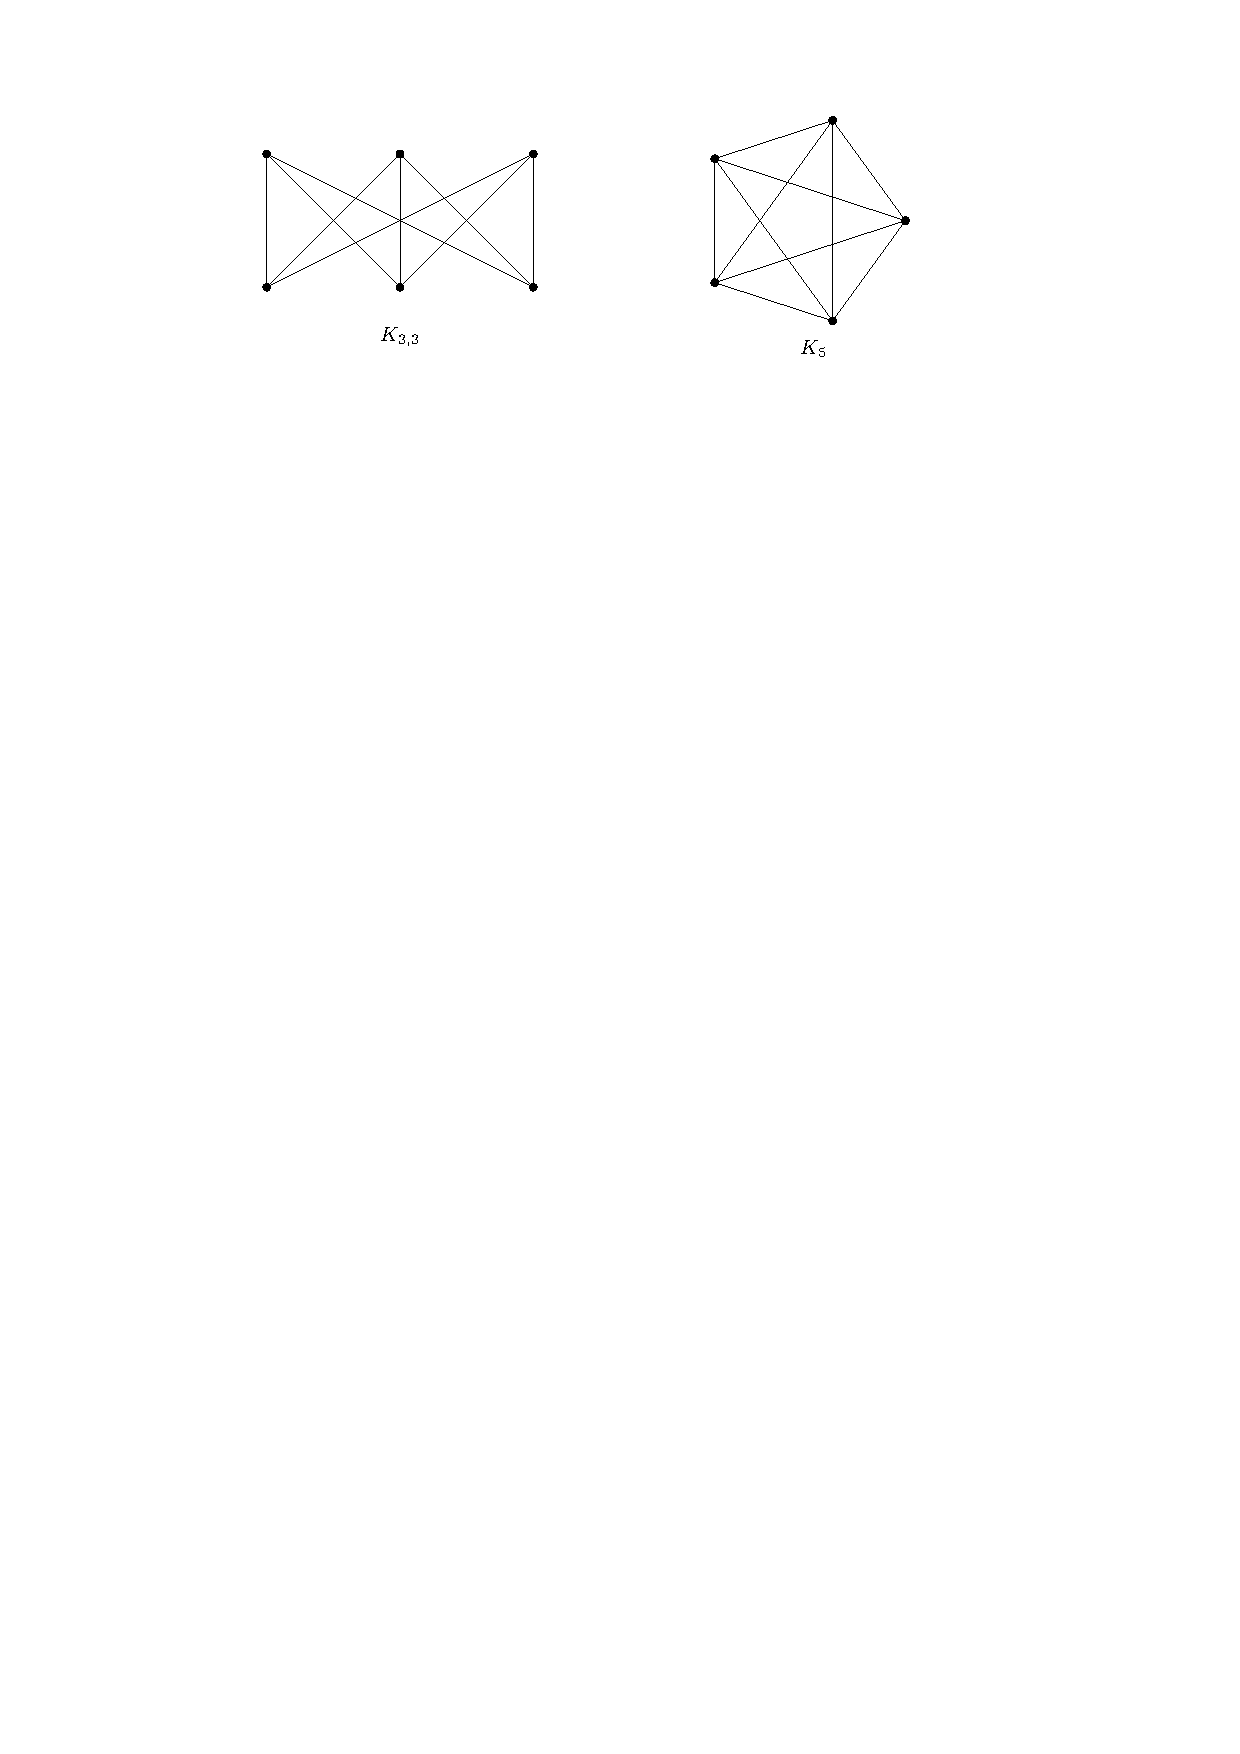
\includegraphics{graphics/kuratowskiExamples.pdf}
\caption{The $K_5$ and $K_{3,3}$ drawn in the plane.}\label{fig:kuratowskiExamples.pdf}
\end{center} 
\end{figure} 
Kuratowski's theorem characterizes finite planar graphs.
A finite graph is planar if and only if it does not contain a subgraph that is a subdivision of $K_5$ or $K_{3,3}$ \cite{kuratowski1930probleme}. 
Figure \ref{fig:kuratowskiExamples.pdf} shows a drawing of $K_5$ and $K_{3,3}$.
Two edges in a drawing \textit{cross} if they have a common interior point.  
The \textit{crossing number} of a graph is the smallest number of edge crossings for a graph over all drawings.
A drawing is said to be \textit{planar} if no two distinct edges cross \cite{BET+99}.
A planar drawing is also called an \textit{embedding}.
Two embeddings of a graph $G$ are \textit{equivalent} if for every vertex the counter-clockwise order of neighbors are the same.% determine the same circular order of the in neighbor sets and the embeddings can be described as a combination of translations and rotations of the other.
A combinatorial \textit{embedding} is a planar drawing with a corresponding counter-clockwise order of the neighbors of each vertex. 
\begin{figure}[!htbp]
\begin{center}
    \includegraphics{graphics/combinatorialEmbedding.pdf}
    \caption{Here is a wheel graph, $W_5$, in two separate drawings with the same counterclockwise ordering of neighbors for each vertex.}\label{fig:combinatorialEmbedding.pdf}
\end{center}
\end{figure}
An orientation preserving rigid transformation (i.e., rotation and translation) map an embedding to an equivalent embedding.  
Reflections reverse the counter-clockwise order around each vertex.

Figure \ref{fig:combinatorialEmbedding.pdf} depicts two different drawings of the wheel graph $W_5$.%, one on the left and one on the right. 
The drawings have the followings counterclockwise order of neighbors for each vertex:
\begin{table}[!htbp]\label{table:combinatorialEmbedding}
\begin{center}
$$\begin{array}{|c|c|c|}\hline
\text{Vertex}&\text{Left \& Middle Drawing}&\text{Right Drawing}\\\hline
1&(2,5,4)& (4,5,2) 
\\\hline
2&(3,5,1) & (1,5,3) 
\\\hline
3&(2,4,5)& (5,4,2) 
\\\hline
4& (1,5,3)  & (3,5,1) 
\\\hline
5&(2,3,4,1)& (4,3,2,1) 
\\\hline
\end{array} $$
\caption{A table showing the counter-clockwise circular ordering of neighbors for the left and right drawing in Figure \ref{fig:combinatorialEmbedding.pdf}.  Note that the permutation cycles are equivalent for the right and left drawings.}
\end{center} 
\end{table}
%The crossing number $cr\lr{\Gamma_G}$ of a drawing of $G$ is the number of crossings in the drawing of the graph $G$. 
%We can treat $cr()$ as a mapping from the space of drawings of $G$ to the non-negative integers, i.e. $cr: \left\lbrace \Gamma_G \right\rbrace \mapsto \bbZ^+ \cup \left\lbrace 0 \right\rbrace$.
%One can ask if for any graph $G$, does there exists a drawing in which the crossing number is zero?
%Without loss of generality, this is a type of crossing number minimization problem, i.e.
%$$ \min_{\gamma \in \left\lbrace \Gamma_G \right\rbrace} cr(\gamma)$$
Referencing table \ref{table:combinatorialEmbedding} and Figure \ref{fig:combinatorialEmbedding.pdf}, we realize that the two drawings of $W_5$ are equivalent.  



%If no two distinct edges intersect in the drawing, the drawing is said to be \textit{planar}. 



 






%Two planar drawings are equivalent if they determine the same circular orderings of the neighbor sets.
%Every proper drawing can be augmented to an embedded plane graph 
%by inserting new vertices at the edge crossings, and subdividing the edges that pass
%through those vertices. So the equivalence of two drawings reduces to the equivalence of plane graphs.


% A graph \textit{embedding} of $G = (V,E)$ is an injective mapping $\Pi: V \mapsto \bbR^2$.  
% \begin{figure}[!htbp]
% \begin{center}
% 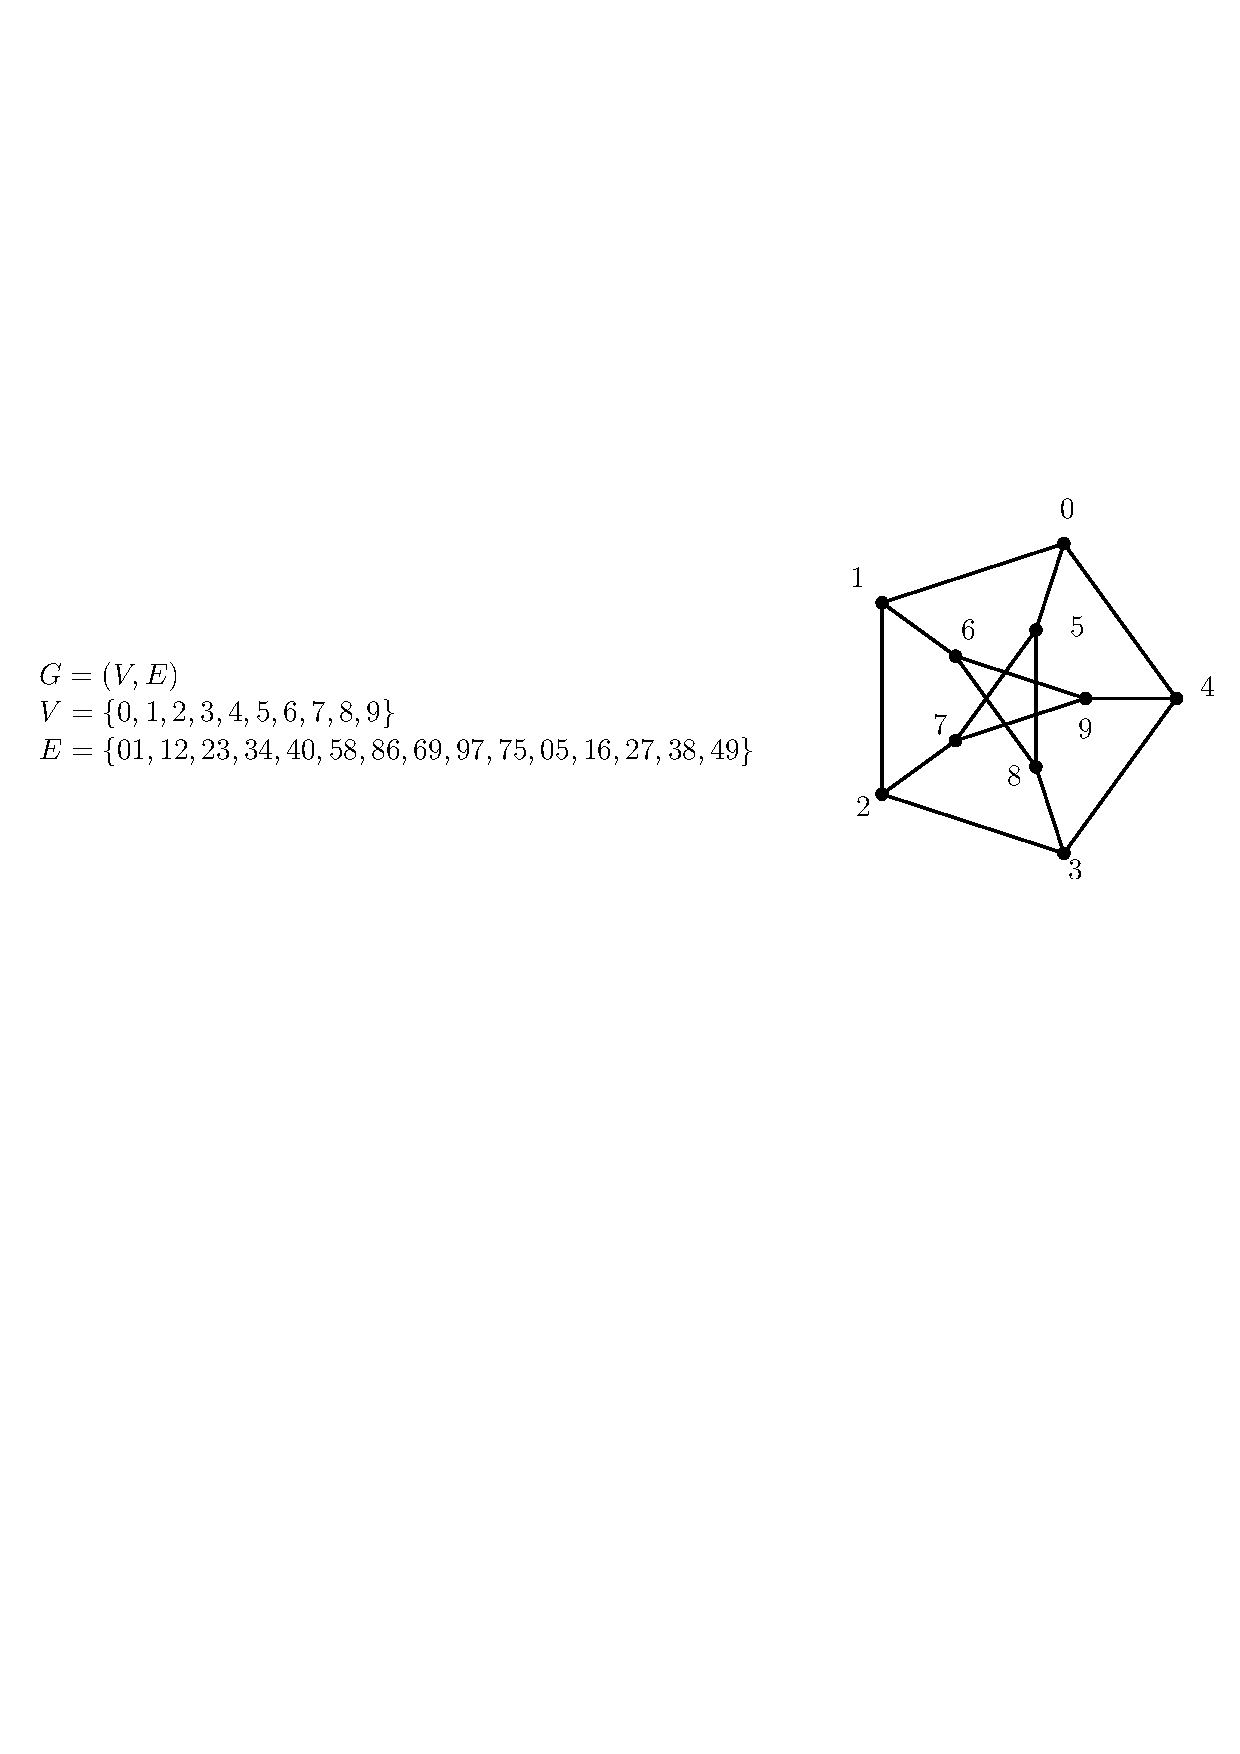
\includegraphics[scale=.5]{graphics/PetersonGraphExample.pdf}
% \caption{An embedding of the Peterson graph.}\label{fig:graph1-1}
% \end{center} 
% \end{figure} 
% A graph embedding is said to


% A \textit{graph} is an 
% ordered pair $G = (V,E)$ comprising of a set of vertices, $V$, and a set of edges or 
% lines, $E$.  Every edge $e \in E$, is an unordered pair of distinct vertices $u,v \in V$ (the edge represents their adjacency, $e = \{ u,v\}$). With this definition of a graph, there 
% are 
% no loops (self adjacent vertices, $\{v,v\}$) or multi-edges (several edges between the same pair of 
% vertices).

%   This requires an 
% embedding into the plane or $\bbr^3$.  An \textit{embedding} of the 
% graph $G = (V,E)$ is an injective mapping $\Pi : V \mapsto \bbR^{2}$ (see Figure 
% \ref{fig:graph1-1}). 


% \subsubsection{Edge Crossings}
% We define \textit{plane embeddings} of a graph to be an embedding where the following degenerate 
% configurations 
% do not occur:
% \begin{itemize}
% \item[\rn{1}] the interiors of two or more edges intersect, or
% \item[\rn{2}] an edge passes through a vertex
% \end{itemize} 
% \begin{figure}[H]
% \begin{center}
%   \begin{subfigure}[b]{0.49\textwidth}
% 	  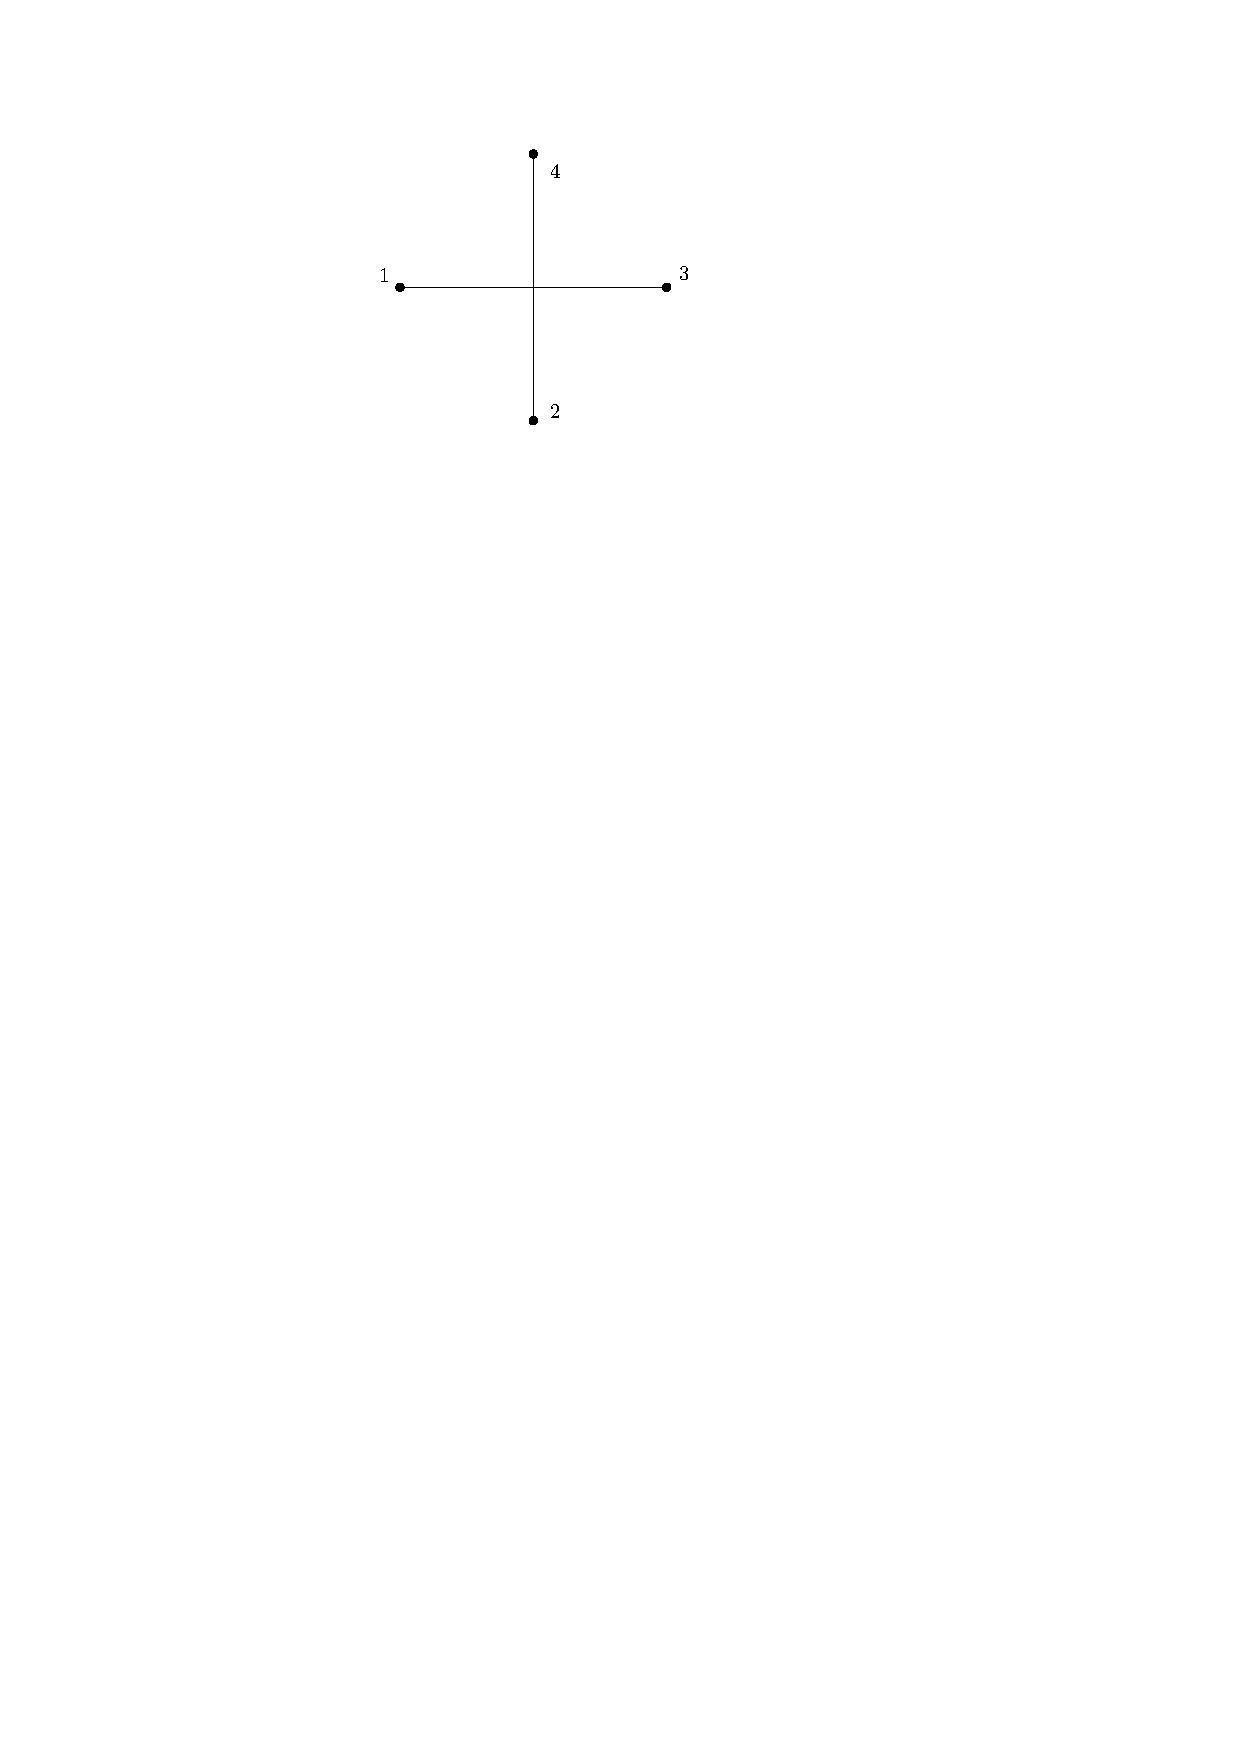
\includegraphics{graphics/crossingType2.pdf}
% 	  \caption{The interior of the edges intersect.}
% 	  \label{fig:ch1-linkages-1-2}
%   \end{subfigure}
%   \begin{subfigure}[b]{0.49\textwidth}
% 	  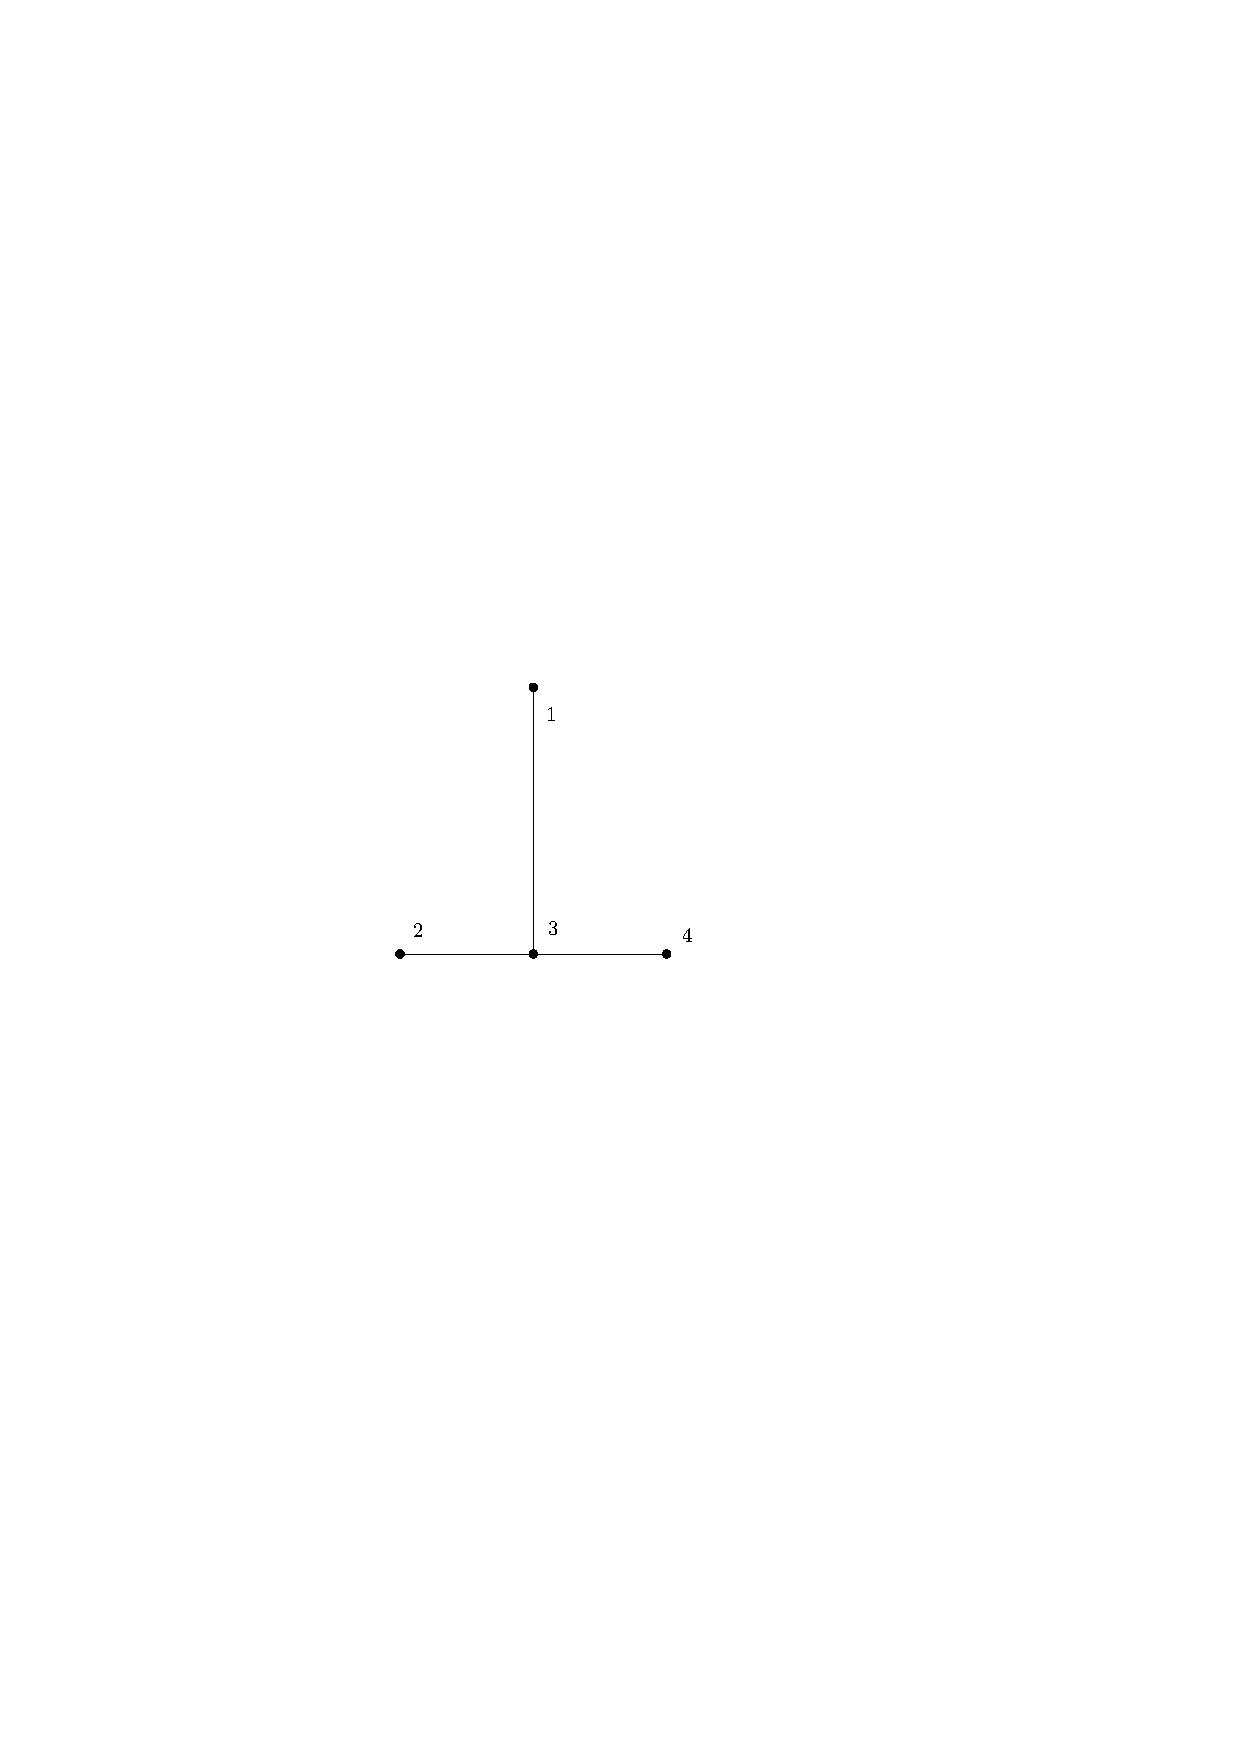
\includegraphics{graphics/crossingType3.pdf}
% 	  \caption{An edge passes through a vertex.}
% 	  \label{fig:ch1-linkages-1-3}
%   \end{subfigure}
% \end{center} 
% \caption{These figures exhibit the 4 types of edge crossings.}\label{fig:ch1-linkages-1}
% \end{figure}
% A graph is called \textit{planar} if it admits a plane embedding.  A \textit{plane graph} is a 
% graph together with a plane embedding.

\subsection{Trees}
%Some graphs can be classified by which properties they have.
A \textit{path} is a sequence of vertices in which every two consecutive vertices are connected by an edge.   
%\begin{figure}[!htbp]
\noindent%
\begin{minipage}{\linewidth}
\begin{center}
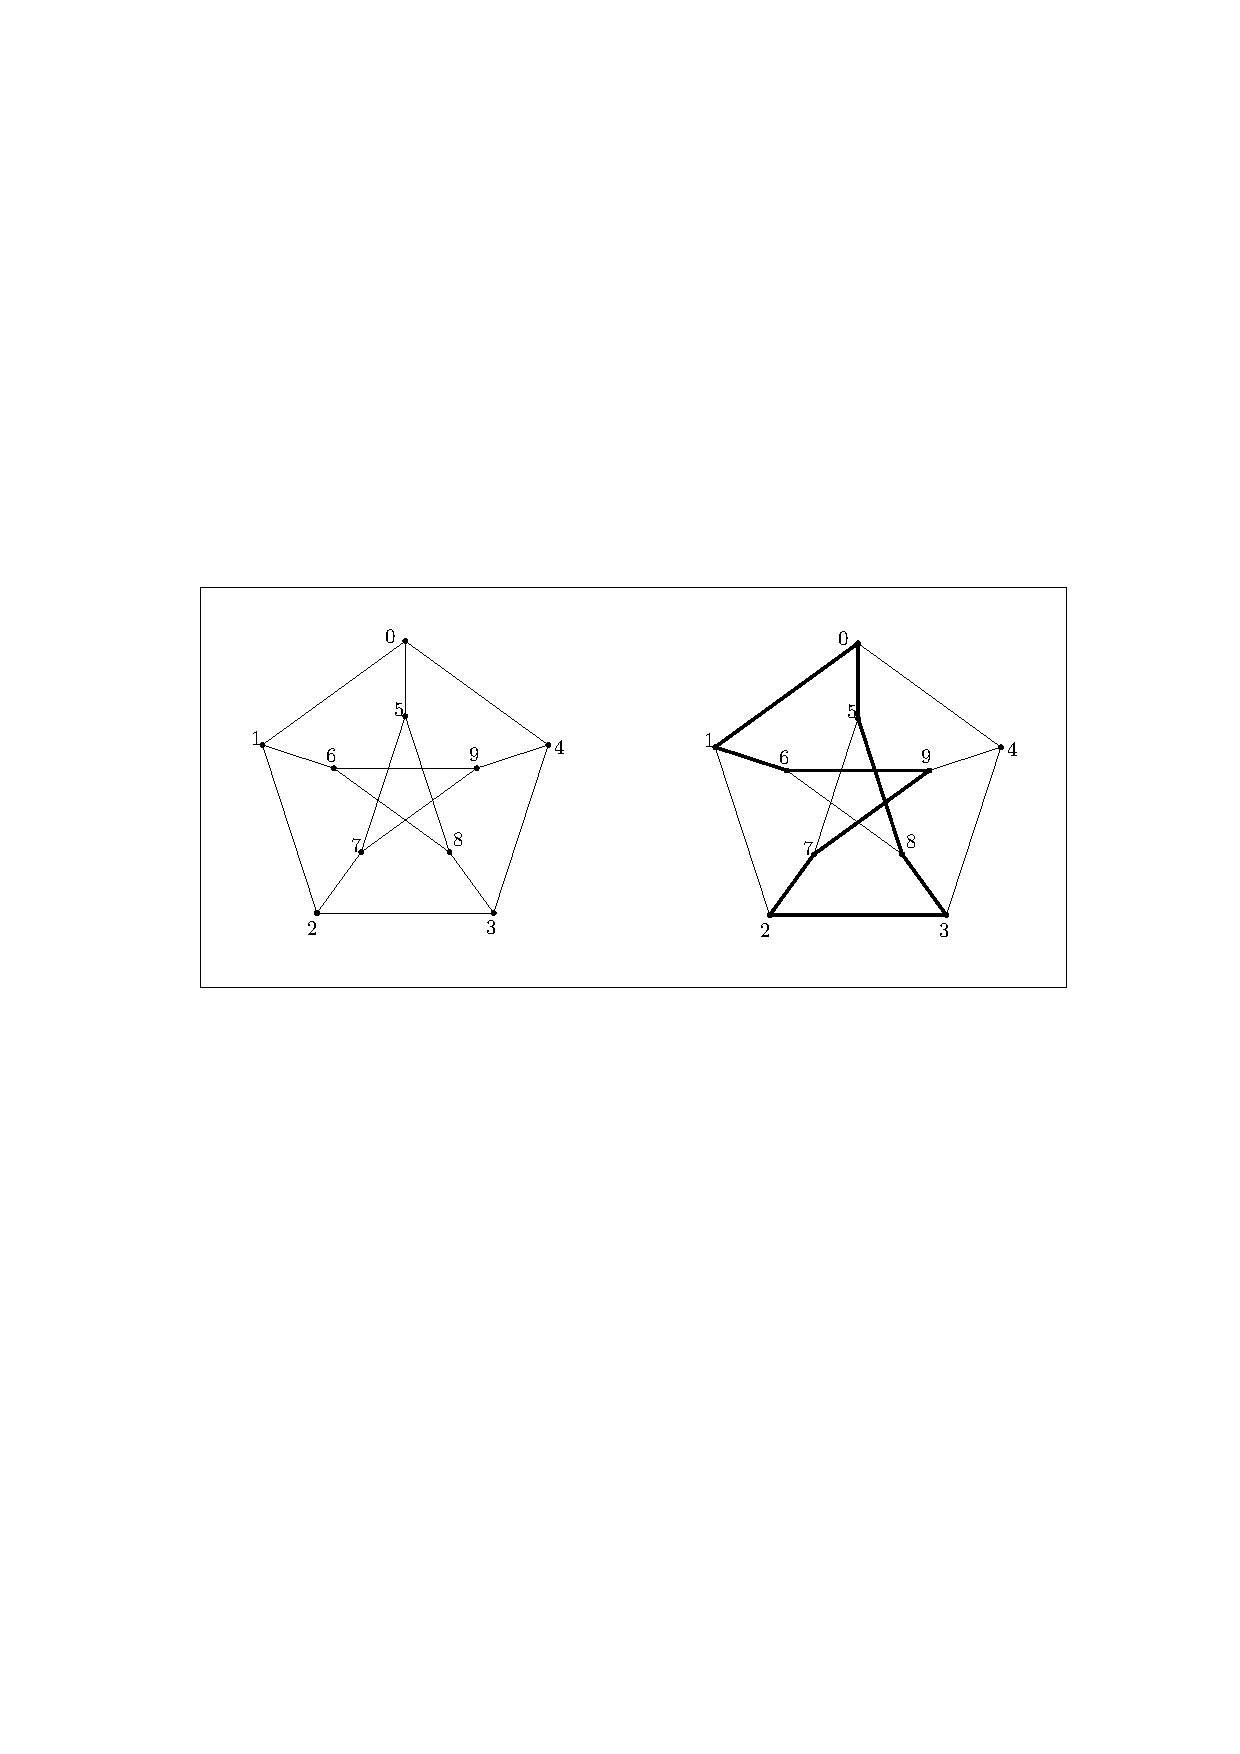
\includegraphics{graphics/PetersonGraphWithPath.pdf}
\captionof{figure}{An embedding of the Peterson graph with a simple cycle of 
(2,7,9,6,1,0,5,8,3).}\label{fig:PetersonGraphWithPath}
\end{center}
%\end{figure}
\end{minipage}
A \textit{simple cycle} of a graph is a sequence, $(v_1, v_2, \dots, v_{t-1},v_t)$, of distinct vertices such that every two consecutive vertices are connected by an edge,  and the last vertex, $v_t$, connects to $v_1$ (see Figure \ref{fig:PetersonGraphWithPath}).  
A graph is \textit{connected} if for any two vertices, there exists a path between the two points.
A \textit{tree} is a graph that has no simple cycles and is connected (see Figure \ref{fig:ch1-graph-2}).
Every tree is planar.
A \textit{forest} is a disjoint union of trees.  
%\begin{figure}[!hbpt]
\noindent%
\begin{minipage}{\linewidth}
\begin{center}
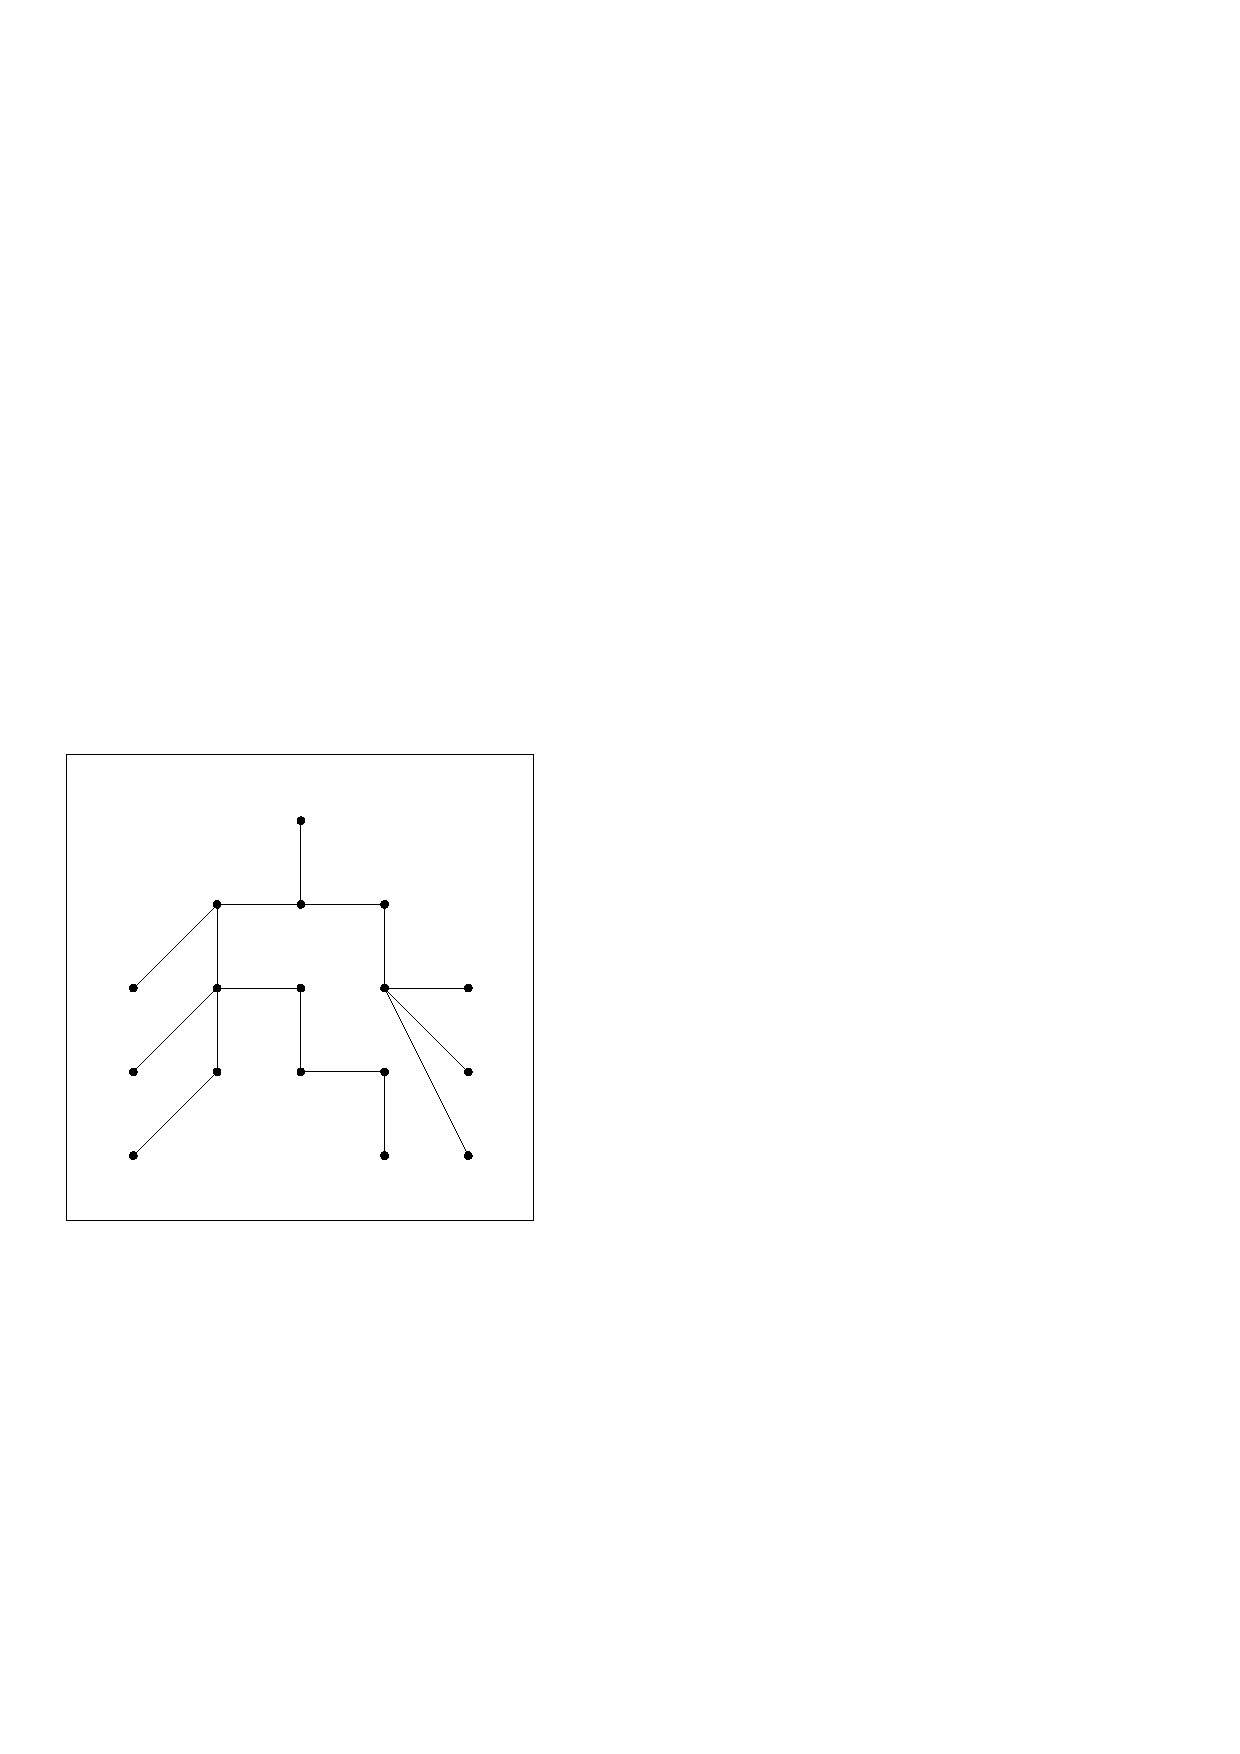
\includegraphics{graphics/RandomTree.pdf}
\captionof{figure}{An example of a tree.}\label{fig:ch1-graph-2}
\end{center}
%\end{figure}
\end{minipage}
%Any two embeddings of trees are equivalent if they can be described as any combination of rotations, translations, and or reflections.

% \subsection{Ordered Trees}
An \textit{ordered tree} is a tree $T$ together with a cyclic order of the neighbors for each vertex (see Figure \ref{fig:ch1-graph-6}).
%\begin{figure}[!hbpt]
\noindent%
\begin{minipage}{\linewidth}
\begin{center}
    \includegraphics{graphics/OrderedTreesExample.pdf}
    \captionof{figure}{A tree with two embeddings with different cyclic orderings around 
vertices.}\label{fig:ch1-graph-6}
\end{center}
%\end{figure}
\end{minipage}

Embeddings of ordered trees are combinatorially equivalent if for each node the counter-clockwise ordering of adjacent nodes are the same. 
%and can be described as a combination of translations and rotations of the other.
%Unlike embeddings for planar graphs where ordering of adjacent vertices is not a distinguishing condition,  we do not consider reflection based transformations for embeddings of ordered trees for equivaliency as that can modify the ordering of adjacent vertices.



% \subsection{Graph Isomorphism} 

% Next we add restrictions to our graph isomorphisms to narrow our focus:
% \begin{itemize}
% \item[\rn{1}] We focus on isomorphisms for planar graphs and or polygonal linkages, simple planar 
% graphs, and
% \item[\rn{2}] the isomorphism preserves edge lengths (polygonal area), e.g. $d(u,v) = d(f(u),f(v))$.
% \end{itemize}  
% With these restrictions of our isomorphisms, we can begin to describe a range of motion to 
% transform a linkage.  That range of motion is said to be the configuration space of that linkage.  
% To expand on this concept, for given linkage, $L=(V,E)$, and for a given vertex $v \in V$, the set 
% of points in which $v$ can be realized in the plane would be the configuration space for that 
% vertex, $C_v$.  Defining some order of the vertices in $L$, i.e. $V = \left\lbrace v_n 
% \right\rbrace_{i=1}^n$, then the \it{configuration space} for $L$ is said to be the cartesion 
% product of the configuration space of vertices:
% \subsection{Summary}
% \begin{table}[!ht]
% \begin{center}
% $$\begin{array}{|l|c|c|}
%  \hline
% &\text{Linkages}&\text{Polygonal Linkages}\\\hline
% \text{Ordered Pair}&G&G\\\hline
% \text{Edges}&E&\HH\\\hline
% \text{Vertices}&V&\PP\\\hline
% l&l&\text{N.A.}\\\hline
% \text{Embedding of }G&\Pi : V \mapsto \bbr^2&\PP ' = \left\lbrace P_i ' 
% \right\rbrace_{i=1}^n\\\hline
% \text{Realization}&\text{See (a)}&\text{See (b)}\\\hline
% \end{array}
% \caption
% $$
% \caption{(a)The realization for a linkage is for any edge $(u,v) \in E$ such that $\left\vert 
% \Pi(u)-\Pi(v)\right\vert = l(u,v)$.(b)A \emph{realization} of a polygonal linkage is an 
% interior-disjoint placement of congruent copies of the polygons in $\PP$ such that the points 
% corresponding to each hinge are identified (Fig. \ref{fig:1}, left).(c).}
% \end{center} 
% \label{table:linkages-2}
% \end{table} 
% %1) 
% %DESCRIBE THE FOLLOWING:
% %1)CONFIGURATION SPACE AS A VECTOR SPACE OF DIMENSION 2^N WHERE EDGE LENGTH IS PRESERVED.
% %2)PINNING 1 VERTEX TO ORIGIN AND A NEIGHBOR, ADD MOTIVATION TO PREVENT ROTATION AND TRANSLATIONS.
% 
% % \begin{equation}\label{eqn:linkages-1}
% % C(L) = C_{v_1} \cross C_{v_2} \cross \cdots \cross C_{v_n}
% % \end{equation} 
% % Some food for thought on configuration spaces and motions on linkages:
% % \begin{itemize}
% % \item[\rn{1}] A configuration space is said to be \it{connected} if there is a continuous mapping 
% for any two planar realizations (linkages) of a graph in the plane.  Otherwise it is said to be 
% \it{disconnected}.
% % \item[\rn{2}] If the configuration space of a vertex, $C_v$, is a singleton set, then the vertex 
% is said to be \it{pinned}. Otherwise it is said to be \it{free}.
% % \item[\rn{3}] The types of motions (mappings) that we refrain from using on linkages are 
% translations.
% % \end{itemize}
% % Note that configuration spaces for polygonal linkages are described similarly.
% % \subsubsection{Realizability of Linkages}
% % Suppose we had two configurations of a linkage, $\mathcal{A}$ and $\mathcal{B}$.  A question that 
% can be posed is can we reconfigure $\mathcal{A}$ to $\mathcal{B}$ continuously while respecting 
% simple planar graph conditions?  The answer to this question is a yes or no.  If yes, then there 
% must exist a path connected configuration space between $\mathcal{A}$ and $\mathcal{B}$.  It has 
% been shown that this problem can be posed as a planar satisfiability problem 
% \cite{Breu19983,mulzer2008minimum} (Later on in this paper we'll cover satisfiability problems).  
% This is the type of problem that we face in this paper.  We will continue to explore this in a 
% different manner, with circle packings.
% \newpage 
